\documentclass[final,t]{beamer}

% themes 
\usetheme{tb2}

% lang
\usepackage[utf8x]{inputenc} \usepackage[english]{babel}

% others
\usepackage{xspace} \usepackage{hyperref} \usepackage{fancyvrb}
\usepackage{listings}
\lstset{language=python, breaklines=true, belowskip=.5em, aboveskip=.5em}

\usepackage[nolist]{acronym}

\usepackage{enumitem} \setitemize{label=\usebeamerfont*{itemize item}%
  \usebeamercolor[fg]{itemize item} \usebeamertemplate{itemize item}}

% graphics
\usepackage{tikz} \usetikzlibrary{arrows} \usetikzlibrary{backgrounds}
\pgfdeclarelayer{background} \pgfdeclarelayer{foreground}
\pgfsetlayers{background,main,foreground}

\graphicspath{{img/}}


% beamer poster !
\usepackage[orientation=portrait,size=a0,scale=2]{beamerposter}

% extra macros
\newcommand{\email}[1]{\texttt{#1}}

% used to set the footer
\newcommand\beamerposterfooter{%
  %\foreach \x in {Python, Silkan_medium, bretagne_cont_quadri}{%
  %  \hfill\includegraphics[height=1.5em]{\x}\hfill%
  %}%
}

\usetikzlibrary{positioning}
\usetikzlibrary{shadows}
\usetikzlibrary{arrows}

% Correct a bug in the vertical spacing by added a 'g' phantom,
% because putting some \strut{} at every line was to much to fit on
% the page...
\title{Pythran: automatic Python to c++ conversion of scientific
  programs}
    

\author{\normalsize  A.~Raynaud \and P.~Brunet \and S.~Guelton}

\institute{\normalsize \vspace{4ex} Journée des utilisateurs de CAPARMOR, Ifremer, Plouzané, 1er février 2013}

\begin{document}

\begin{frame}[fragile]

    \vspace{-.5em}

    \begin{columns}
        % 
        \column{.03\textwidth}{}

        \column{.45\textwidth}{
            \Large
            \begin{itemize}
                \item A \textbf{Python to C++} compiler for a subset of the
                    Python language.
                \item Makes numerical algorithms written in Python run faster.
            \end{itemize}
            \vspace{-1em}
        }

        \column{.04\textwidth}{}

        \column{.45\textwidth}{
            \Large
            \begin{itemize}
                \item Turns sequential programs into multithreaded
                    ones using well-known \textbf{OpenMP} directives.
            \end{itemize}
        }

        \column{.03\textwidth}{}

    \end{columns}

    \vspace{\baselineskip}

    \begin{block}{\Large Pythran Language $\subset$ Python Language}

        \vspace{-.5em}

        \begin{columns}
            \column{.03\textwidth}{}

            \column{.4\textwidth}{
                \Large
                \begin{itemize}
                    \item Implicitly \textbf{statically typed}
                    \item list, set, dict, [numpy array]
                    \item import math, random, [numpy]
                    \item generators, comprehension
                    \item \textbf{No} User Class
                \end{itemize}
            }

            \column{.04\textwidth}{}

            \column{.5\textwidth}{
                \Large
                \begin{itemize}
                    \item Open Source Software (BSD License)
                    \item Source Repository on github:
                        {\normalsize\texttt{https://github.com/serge-sans-paille/pythran}}

                    \item Freenode: \texttt{\#pythran}
                    \item Mliste: \texttt{pythran@freelists.org}
                \end{itemize}
            }

            \column{.03\textwidth}{}
        \end{columns}
    \end{block}

    \begin{block}{\Large Pythran Compilation}

        \vspace{-.5em}

        \begin{columns}

            \column{0.01\textwidth}{}

            \column{0.39\textwidth}{

                \vspace{\baselineskip}

                \begin{tikzpicture}[
                        file/.style={draw=tbgreen!50,fill=tbgreen!10,rectangle, drop shadow, align=center},
                    tool/.style={draw=tbgreen!50,fill=tbgreen!10,circle, align=center}]
                    \node[file] (python) {\textbf{Python Module [\texttt{.py}]}};
                    \node[file] (annotation)	   [right=of python] {\textbf{Type Info}};
                    \node[file] (omp)	   [left=of python] {\textbf{OpenMP}};
                    \node[tool] (pythran) [below=of python] {\textbf{Pythran}};
                    \node[file] (cxx) [below=of pythran] {\textbf{C++}};
                    \node[file] (boost) [left=of cxx] {\textbf{\texttt{boost::python}}};
                    \node[file] (pythonic) [right=of cxx] {\textbf{\texttt{pythonic++}}};
                    \node[tool] (gxx) [below=of cxx] {\textbf{g++}};
                    \node[file] (so) [below=of gxx] {\textbf{Native Module [\texttt{.so}]}};

                    \draw[very thick, ->] (python) -- (pythran);
                    \draw[very thick,dashed, ->] (annotation) -- (pythran);
                    \draw[very thick,dashed, ->] (omp) -- (pythran);
                    \draw[very thick, ->] (pythran) -- (cxx);
                    \draw[very thick, ->] (cxx) -- (gxx);
                    \draw[very thick, ->] (boost) -- (gxx);
                    \draw[very thick, ->] (pythonic) -- (gxx);
                    \draw[very thick, ->] (gxx) -- (so);
                \end{tikzpicture}

            }
            \column{0.04\textwidth}{}   

            \column{0.45\textwidth}{   

                \begin{lstlisting}[language=python]
#pythran export pi_estimate(int)
def pi_estimate(DARTS):
 hits = 0
 "omp parallel for private(x,y,dist), reduction(+:hits)"
 for i in xrange (0, DARTS):
  x = random()
  y = random()
  dist = sqrt(pow(x, 2) + pow(y, 2))
  if dist <= 1.0:
   hits += 1.0
 pi = 4 * (hits / DARTS)
 return pi
\end{lstlisting}

            }

            \column{0.01\textwidth}{}   

        \end{columns}
        \vspace{-.5\baselineskip}

    \end{block}


    \begin{block}{\Large Sequential and Parallel Speedup }

        %\vspace{\baselineskip}

        \begin{columns}

            \column{0.45\textwidth}{
                \vspace{0.4\baselineskip}
                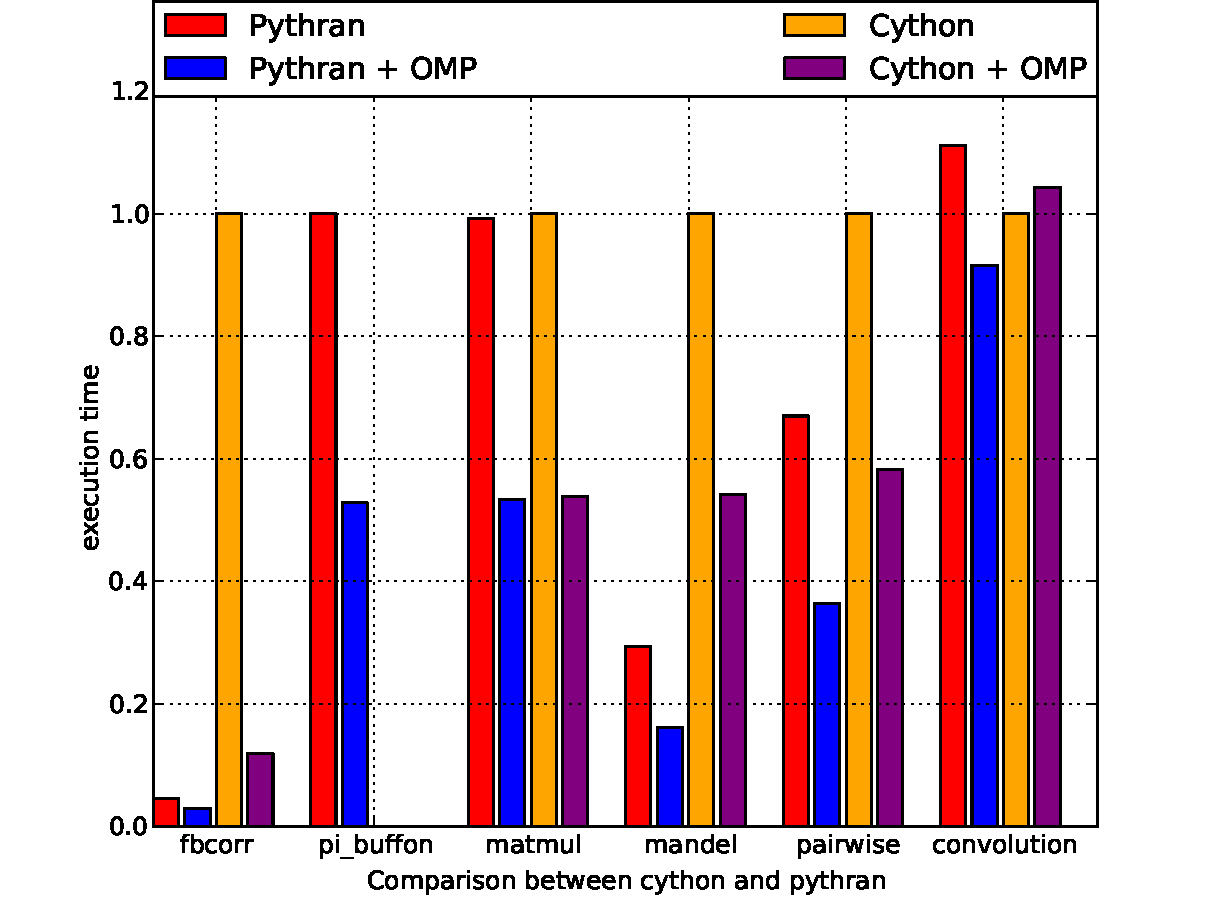
\includegraphics[width=\textwidth]{cython}
            }

            \column{0.55\textwidth}{ 
                \vspace{0.4\baselineskip}

                \begin{itemize}
                    \item \large Pythran outperforms CPython, the
                        standard implementation of Python.
                        \begin{itemize}
                                %\normalsize
                            \item Up to 2000x faster.
                            \item Additional boost whith parallelism.
                        \end{itemize}
                        \vspace{0.4\baselineskip}
                    \item \large Pythran generates faster code than other Python
                        optimization tools, like PyPy, Shedskin or Cython.
                \end{itemize}

                \vspace{\baselineskip}

                \foreach \x in {python, Silkan_medium, bretagne_cont_quadri}{
                    \includegraphics[height=3.5em]{\x}\hfill
                }

            }

        \end{columns}

    \end{block}


\end{frame}

\end{document}

%%% Local Variables:
%%% mode: latex
%%% mode: tex-pdf
%%% mode: flyspell
%%% ispell-local-dictionary: "american"
%%% End:
